\section{Scheduling}
\begin{itemize}
	\item static vs. dynamic
	\item preemptive vs. non-preemptive
	\item with vs. without resource constrains
	\item aperiodic vs. periodic (iterative)
\end{itemize}

\subsection{Scheduling without resource constrains}
\begin{itemize}
	\item ASAP (as soon as possible)
\begin{itemize}
	\item determines the earliest start times of tasks
	\item computes the minimal latency
\end{itemize}
\item ALAP (as late as possible)
\begin{itemize}
	\item determines the latest start times of tasks (for a given latency bound) 
\end{itemize}
\item Mobility of a tsk is given by the difference between ALAO and ASAP start times
\begin{itemize}
	\item Mobility 0 $\rightarrow$ task on critical path
\end{itemize}
\end{itemize}

\subsection{Definition}
\subsubsection{Definition: Schedule}
A schedule of a sequencing graph $G_S = (V_S, E_S)$ is a function $\tau: V_S \rightarrow \N$ that satisfies:
$$
	\tau(v_j) - \tau(v_i) \geq d_i \quad \forall(v_i, v_j)\in E_S
$$ 

\subsubsection{Definition: Latency}
The latency $L$ of a schedule $\tau$ of a sequencing graph $G_S = (V_S, E_S)$ is defined as:
$$
	L = \max_{v_i \in V_S} \{\tau(v_i) + d_i\} - \min_{v_j \in V_S} \{\tau(v_j)\}
$$
And therefore denotes the number of tine steps of the smallest time interval that includes the execution of all nodes $v_i \in V_S$

\subsection{ASAP}
\begin{figure}[h]
	\begin{center}
		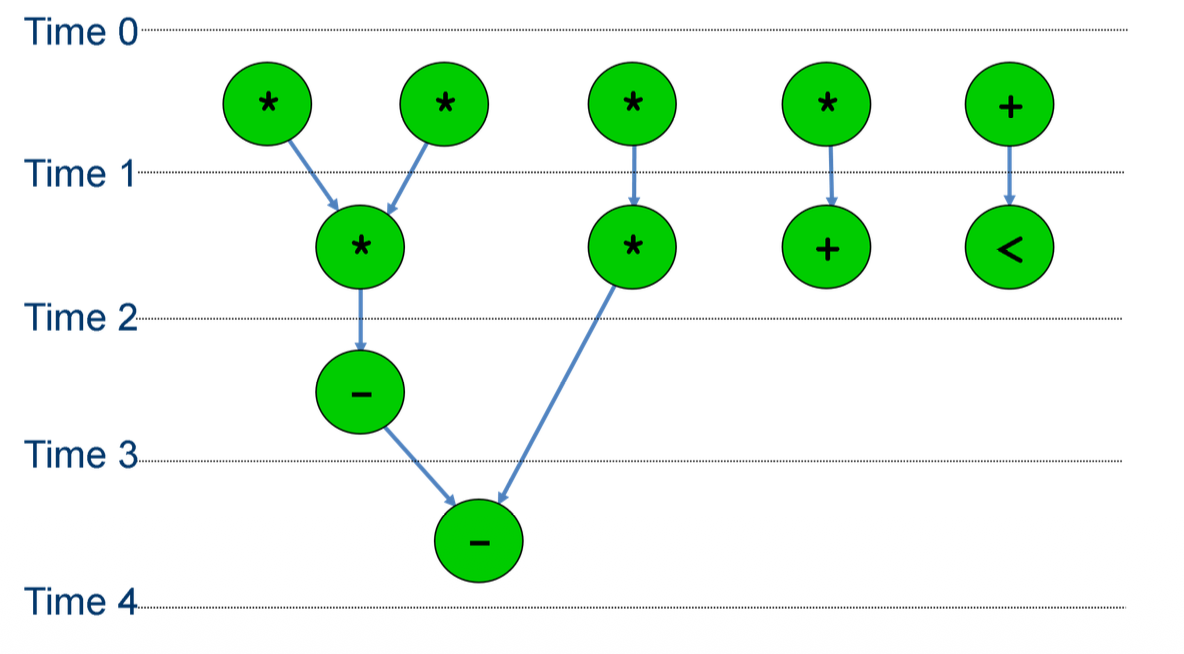
\includegraphics[width=0.5\textwidth]{images/ASAP_graph.png}
		\caption{latency-optimal schedule: $L = 4$}
		\label{fig:ASAP_graph}
	\end{center}
\end{figure}
\begin{figure}[h]
	\begin{center}
		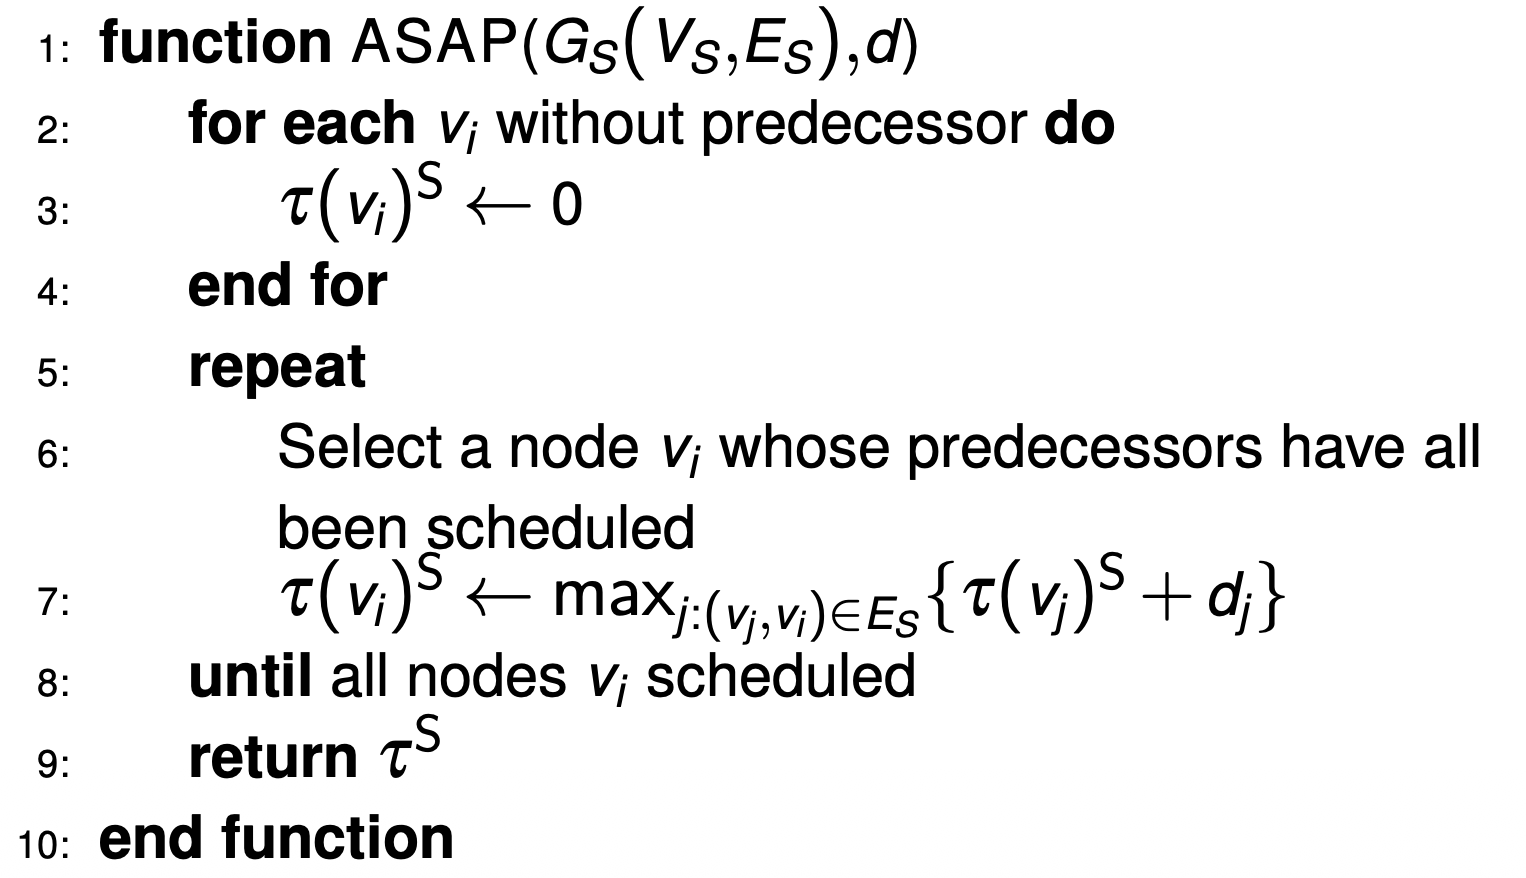
\includegraphics[width=0.5\textwidth]{images/ASAP.png}
		\caption{ASAP algorithm}
		\label{fig:ASAP_algo}
	\end{center}
\end{figure}

\subsection{ALAP}
\begin{figure}[h]
	\begin{center}
		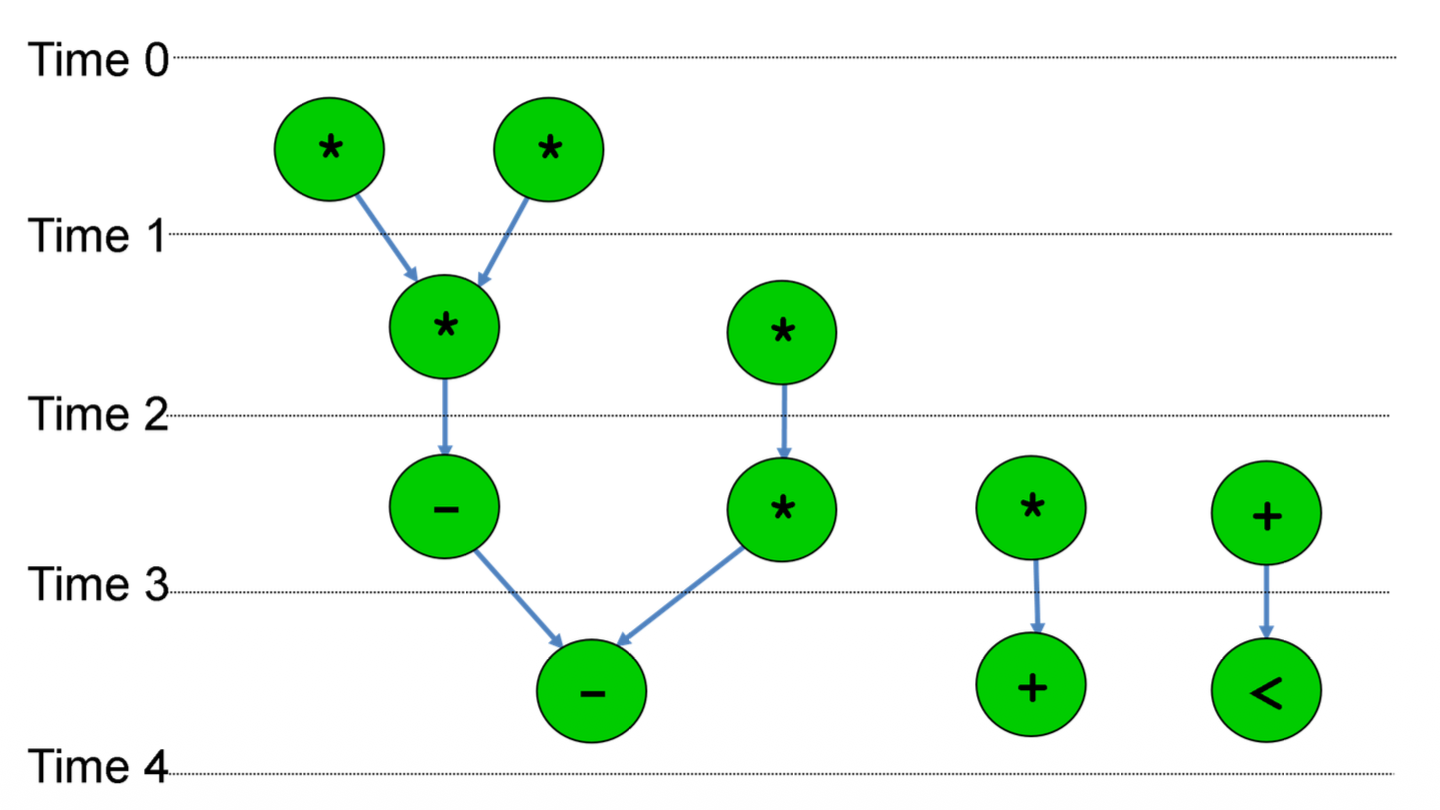
\includegraphics[width=0.5\textwidth]{images/ALAP_graph.png}
		\caption{latency bound: $\overline L = 4$}
		\label{fig:ALAP_graph}
	\end{center}
\end{figure}

\begin{figure}[h]
	\begin{center}
		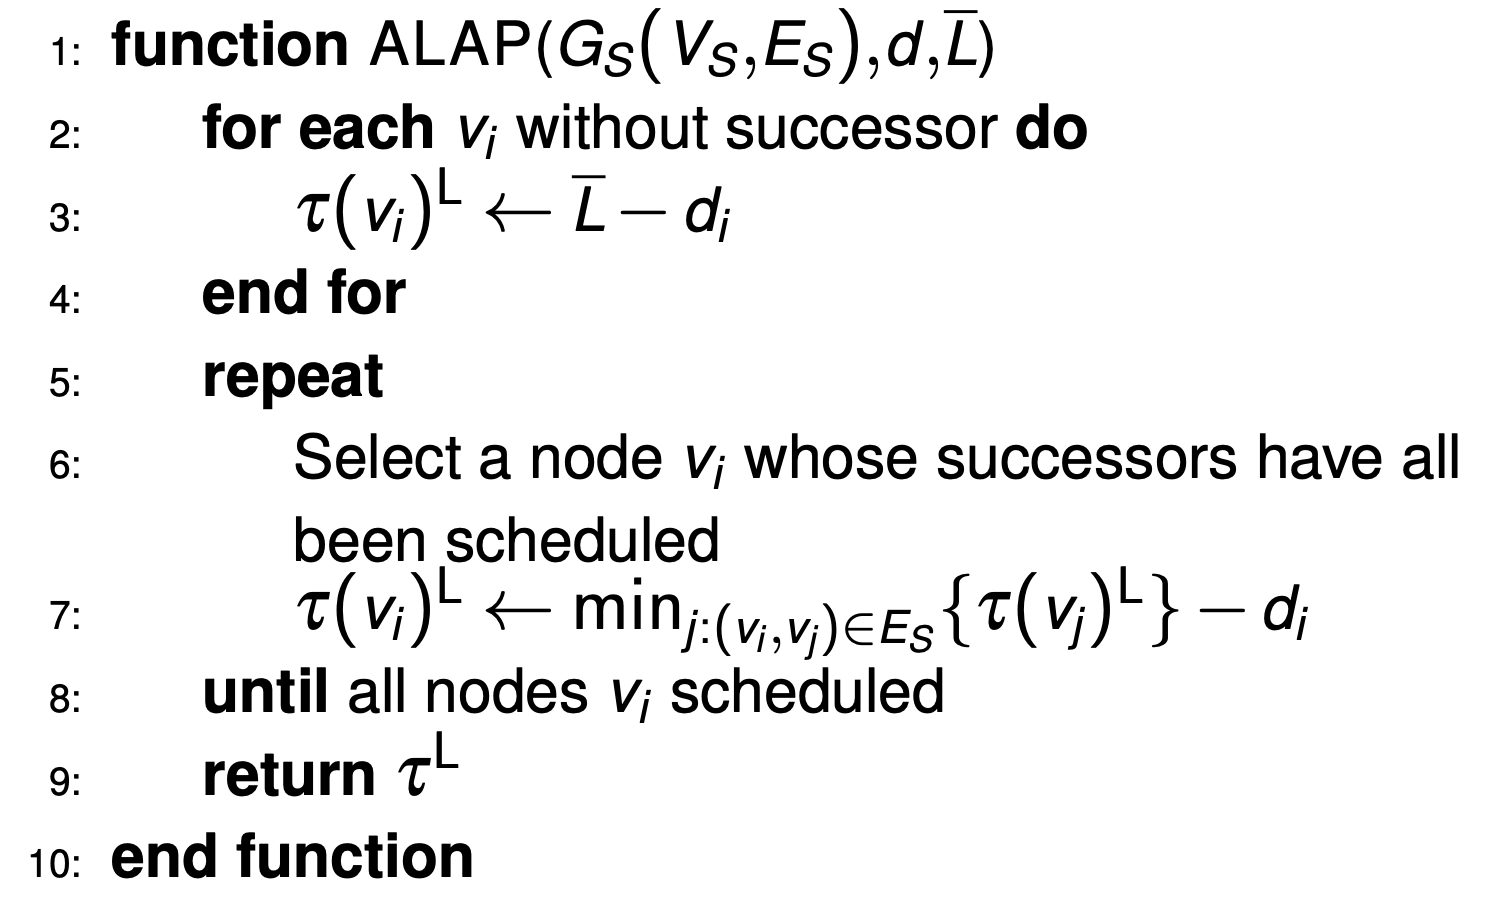
\includegraphics[width=0.5\textwidth]{images/ALAP.png}
		\caption{ALAP algorithm}
		\label{fig:ALAP_algo}
	\end{center}
\end{figure}

\subsection{List scheduling}
\begin{itemize}
	\item Task are sorted into a list according to some priority function
	\item In each step, each free resource will be assigned a schedulable task of highest priority
	\item Priority functions: number of successor nodes, mobility, \dots
\end{itemize}

\begin{figure}[h]
	\begin{center}
		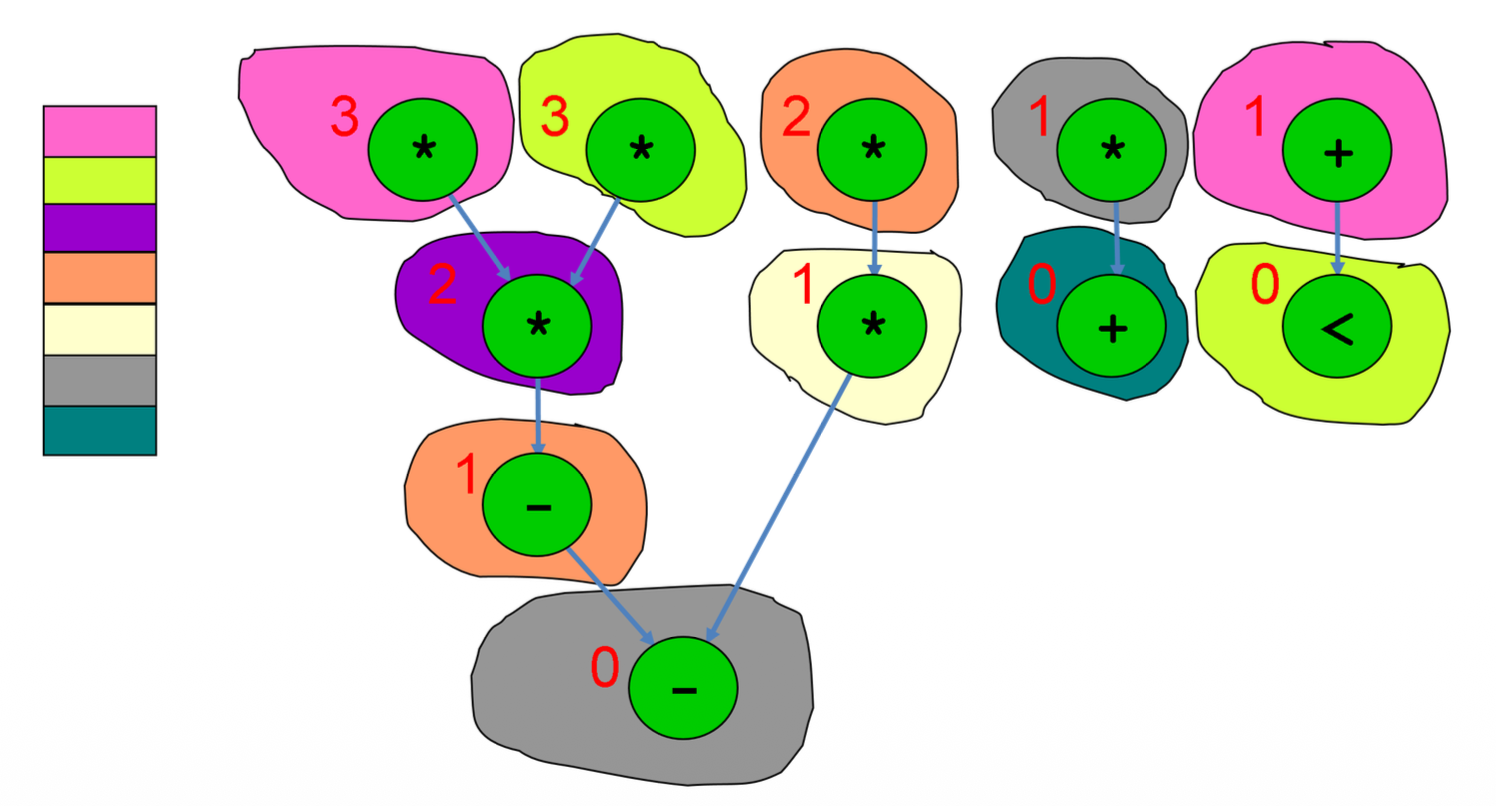
\includegraphics[width=0.5\textwidth]{images/List_scheduling_graph.png}
		\caption{Priority: Number of successor nodes \\
		Resources: 1 multiplier, 1 ALU (+, -, $<$)}
		\label{fig:list_scheduling_graph}
	\end{center}
\end{figure}

\begin{figure}
	\begin{center}
		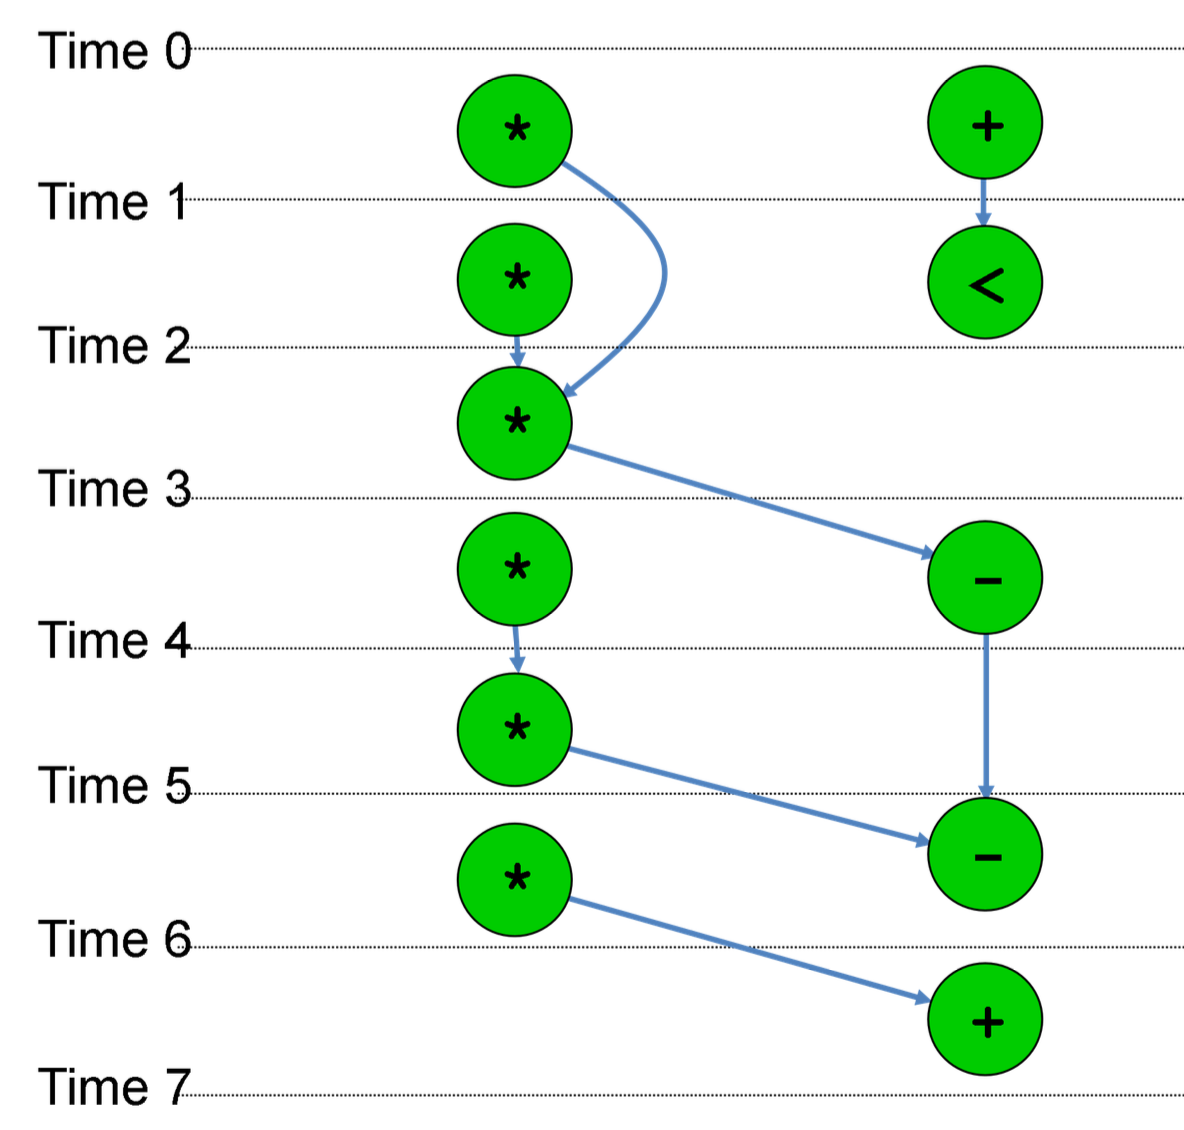
\includegraphics[width=0.5\textwidth]{images/List_scheduling.png}
		\caption{List scheduling}
		\label{fig:list_scheduling}
	\end{center}
\end{figure}

\subsection{Periodic scheduling}

\begin{figure}
	\begin{center}
		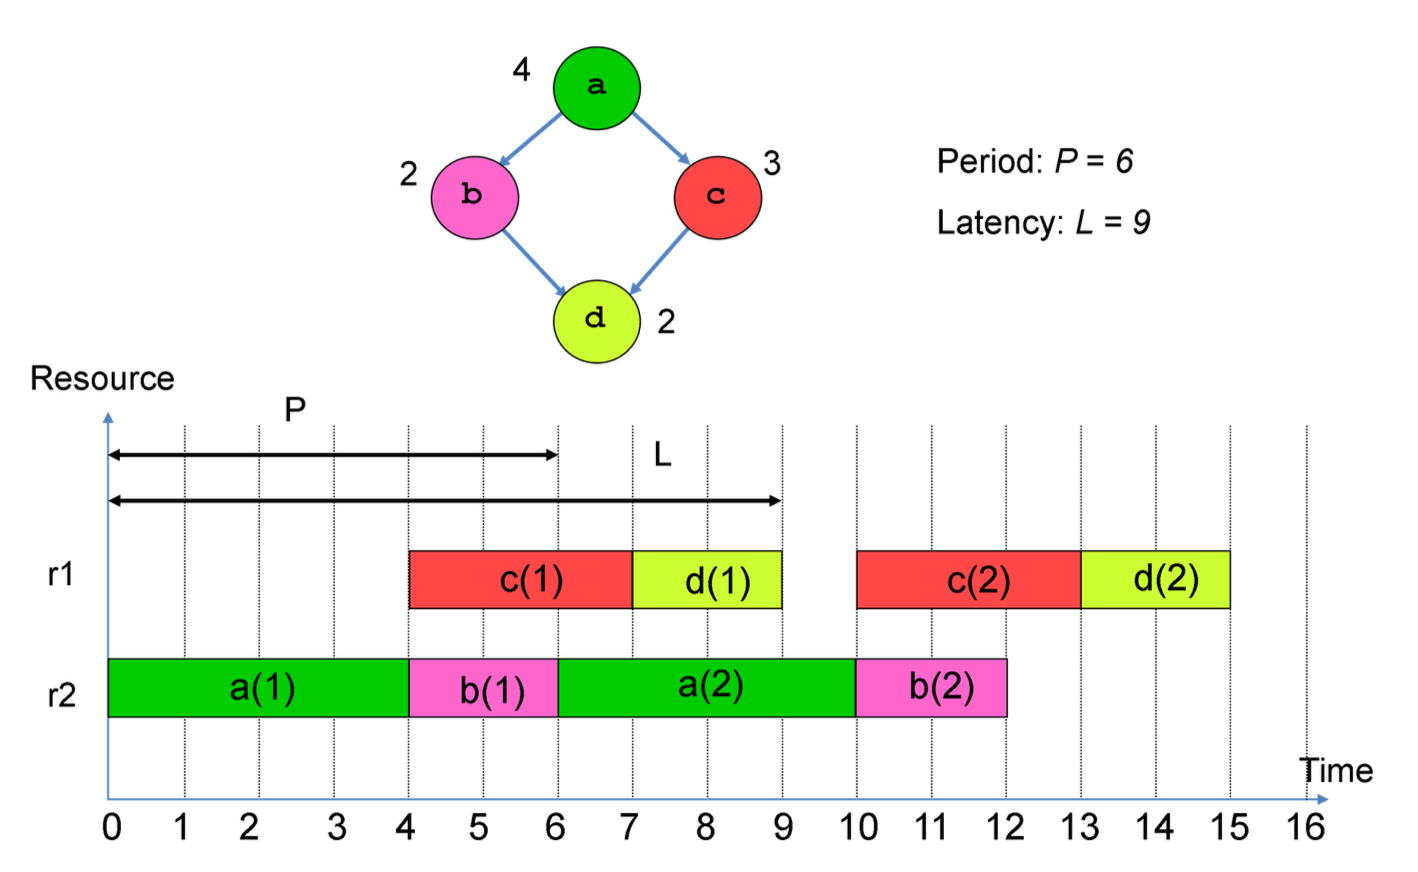
\includegraphics[width=0.5\textwidth]{images/Periodic_scheduling.png}
		\caption{Periodic scheduling}
		\label{fig:periodic_scheduling}
	\end{center}
\end{figure}






